\documentclass{beamer}
\usetheme{Warsaw}
\usecolortheme{beaver}
\title[Bias, Variance and Parsimony in Regression Analysis]{Bias, Variance and Parsimony in Regression Analysis\\ECS 256 Winter 2014}
\author[Matloff]{
Christopher Patton, \texttt{cjpatton@ucdavis.edu}\\
Alex Rumbaugh, \texttt{aprumbaugh@ucdavis.edu}\\
Thomas Provan,\texttt{tcprovan@ucdavis.edu}\\
Olga Prilepova, \texttt{prilepova@gmail.com}\\
John Chen, \texttt{jhochen@ucdavis.edu}}
\institute{ECS 256, Winter 2014\\ \Large{UC Davis}}
\date{March 12, 2014}
\begin{document}

\begin{frame}
\titlepage
\end{frame}


\begin{frame}{Introduction}
This is the introduction.
\end{frame}

% Alex's Section -----------------------------------------------------------------

\begin{frame}
    \frametitle{California Housing Data}
\end{frame}

\begin{frame}
    \frametitle{Parsimony}
\end{frame}

\begin{frame}
    \frametitle{Regression Coefficients}
\end{frame}

\begin{frame}
    \frametitle{Latitude \& Longitude}
\end{frame}

\begin{frame}
    \frametitle{Understanding}
\end{frame}

\begin{frame}
%Image of Plots Here
\end{frame}

\begin{frame}
%Image of Plots Here
\end{frame}

\begin{frame}
%Image of Plots Here
\end{frame}

% End Alex's Section--------------------------------------------------------------

% Olga's Section--------------------------------------------------------------


\begin{frame}
\frametitle{Census Based on 1994}
\end{frame}

\begin{frame}
\frametitle{Age}
\end{frame}

\begin{frame}
\frametitle{}

\begin{figure}
 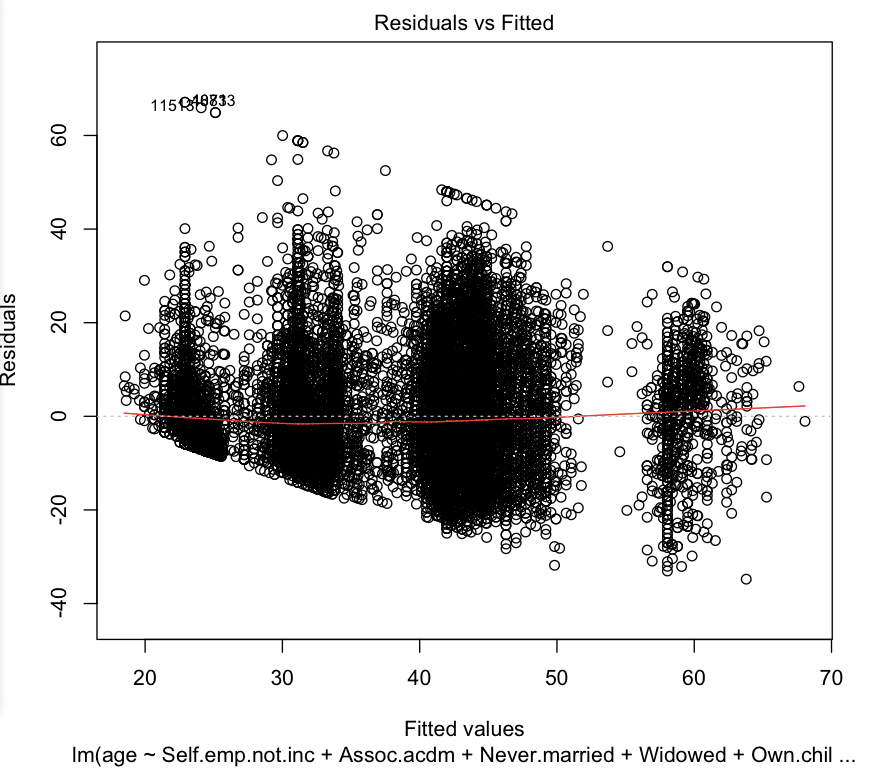
\includegraphics[scale=0.3]{figures/ageResidCensus.png}
 \label{fig:ageResidCensus}
\end{figure}
 
\end{frame}

\begin{frame}
\frametitle{Census Based on 1994}
% Census Sex Coefficients
\end{frame}

\begin{frame}
\frametitle{Census Based on 1994}
% Census Salary Coefficients
\end{frame}

\begin{frame}
%Picture of predicted vs actual age
\begin{figure}
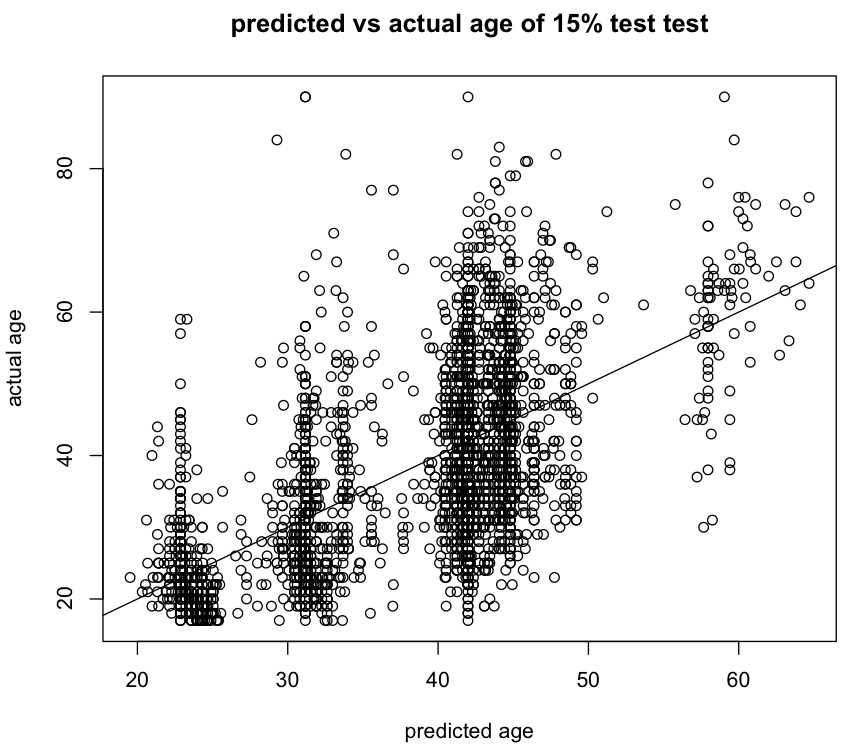
\includegraphics[scale=0.3]{figures/predVsActualCensus.png}
\label{fig:predVsActualCensus}
\end{figure}
\end{frame}

\begin{frame}
%Picture of predicted vs actual age

\begin{figure}
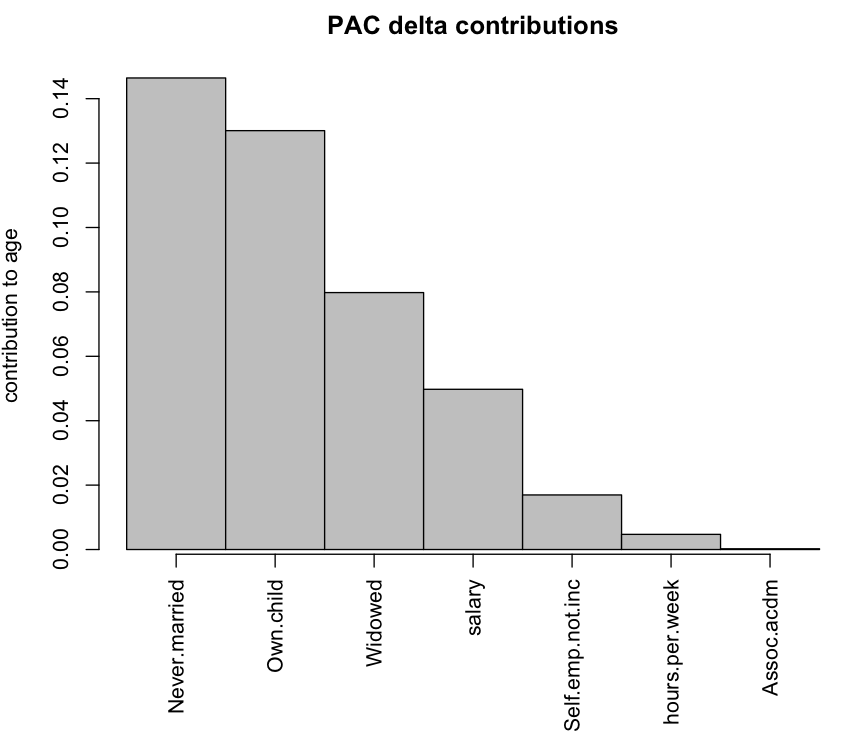
\includegraphics[scale=0.3]{figures/ageContrib.png}
\caption{}
 \label{fig:ageContrib}
\end{figure}

\end{frame}
% End Olga's Section--------------------------------------------------------------

% Begin Chris' Section--------------------------------------------------------------


\begin{frame}
\frametitle{}
%Slide 1
\end{frame}

\begin{frame}
\frametitle{}
%Slide 2
\end{frame}

\begin{frame}
\frametitle{}
%Slide 3
\end{frame}

\begin{frame}
\frametitle{}
%Slide 4
\end{frame}

\begin{frame}
\frametitle{}
%Slide 5
\end{frame}

% End Chris' Section--------------------------------------------------------------
% Thomas' Section--------------------------------------------------------------


\begin{frame}
\frametitle{}
%Slide 1
\end{frame}

\begin{frame}
\frametitle{}
%Slide 2
\end{frame}

\begin{frame}
\frametitle{}
%Slide 3
\end{frame}

\begin{frame}
\frametitle{}
%Slide 4
\end{frame}

\begin{frame}
\frametitle{}
%Slide 5
\end{frame}
% End Thomas' Section--------------------------------------------------------------
% John's Section--------------------------------------------------------------


\begin{frame}
\frametitle{}
%Slide 1
\end{frame}

\begin{frame}
\frametitle{}
%Slide 2
\end{frame}

\begin{frame}
\frametitle{}
%Slide 3
\end{frame}

\begin{frame}
\frametitle{}
%Slide 4
\end{frame}

\begin{frame}
\frametitle{}
%Slide 5
\end{frame}
% End John's Section--------------------------------------------------------------
\end{document}